\documentclass{beamer}
\usepackage[spanish]{babel}
\usepackage[utf8]{inputenc}
\usepackage{graphicx}
\usepackage{color}
\newtheorem{definicion}{Definición}
\newtheorem{ejemplo}{Ejemplo}

%%%%%%%%%%%%%%%%%%%%%%%%%%%%%%%%%%%%%%%%5

\usetheme{Madrid} 
\usecolortheme{crane}
%%%%%%%%%%%%%%%%%%%%%%%%%%%%%%%%%%%%%%%%%%%%%%%%%%%%%%%%%%%%%%

\title{Polinomio de Taylor}
\author{{Jennifer Cabrera Mesa} \\ {Claudio García Vargas} \\ {Lorena Díaz Morales} \\ \bigskip {Universidad de La Laguna}}
\date{17 de Mayo 2013}

%%%%%%%%%%%%%%%%%%%%%%%%%%%%%%%%%%%%%%%%%%%%%%%%%%%%%%%%%%%%%%%%

\begin{document}
%portada
\begin{frame}[plain]
\begin{center}
 
\includegraphics[width=0.2 \textwidth]{brook-taylor.eps}
\end{center}

\titlepage
\end{frame}

%indice
\begin{frame}
\frametitle{Indice}
\small
\tableofcontents[pausesections]
\end{frame}

\AtBeginSubsection[]
{
\begin{frame}{Indice}
\tableofcontents[currentsection,currentsubsection]
\end{frame}
}
%%%%%%%%%%%%%%%%%%%%%%%%%%%%%%%%%%%%%%%%%%%%%%%%%%%%%%%%%%%%%%%%%%%%%%%%%%%%%%%%%%%%%%%%%%%

\section{Motivación y objetivos}
\subsection{Justificación del trabajo}
\begin{frame}
\frametitle{Justificación del trabajo}
\begin{itemize}
 \item
    Objetivo principal : Implementación en python del desarrollo de Taylor.
 \item
    Objetivo especifico : Como se comporta la interpolación de una función logaritmica.
\end{itemize}
Las ventajas que tiene este metodo de aproximacion:
\begin{itemize}
 \item 
    La derivacion del polinomio se puede realizar termino a termino lo que hace que resulten operaciones triviales. 
 \item
    Se puede utilizar para calcular valores aproximados de la funcion.
 \item
    Si es posible transformar una funcion mediante el polinomio de Taylor se comprueba que seria la aproximacion optima posible. 
\end{itemize}
\end{frame}

%%%%%%%%%%%%%%%%%%%%%%%%%%%%%%%%%%%%%%%%%%%%%%%%%%%%%%%%%%%%%%%%%%%%%%
\subsection{Objetivos}
\begin{frame}
\frametitle{Objetivos}
\begin{itemize}
 \item 
    Implementación en python para calcular el desarrollo en serie de Taylor para la función f(x)=ln(6x), x $\in$ [1,7]
 \item
    Adquirir práctica a la hora de redactar documentos científicos con latex.
 \item
    Realizar presentaciones con beamer para la exposición en público.
 
\end{itemize}
\end{frame}

%%%%%%%%%%%%%%%%%%%%%%%%%%%%%%%%%%%%%%%%%%%%%%%%%%%%%%%%%%%%%%%%%%%%%%%%%%%
\section{Fundamentos teóricos}
\subsection{Notas históricas sobre el polinomio de Taylor}
\begin{frame}
 \frametitle{Fundamentos teóricos}
 \begin{itemize}
  \item Zenón de Elea
  \item Demócrito y Arquímedes 
  \item Madhava de Sangamagrama
  \item James Gregory 
  \item Brook Taylor
 \end{itemize}

\end{frame}

%%%%%%%%%%%%%%%%%%%%%%%%%%%%%%%%%%%%%%%%%%%%%%%%%%%%%%%%%%%%%%%%%%%%%%%%%%%%%

\subsection{Fórmula de Taylor}
\begin{frame}
 \frametitle{Fórmula de Taylor}

\begin{displaymath}
f(x) = f(a)+f'(a)(x-a) + \frac{f^{(2)}(a)}{2!}(x-a)^2 + \ldots{} + \frac{f^{(n)}(a)}{n!}(x-a)^n
\end{displaymath}

Expresado como sumatorio, queda de la siguiente forma

\begin{displaymath}
\sum_{n=0}^\infty\frac{f^{(n)}(a)}{n!}(x-a)^{n}
\end{displaymath}

Añadiendo el resto a la expresión:

\begin{displaymath}
f(x) = P_n(x;a) + R_n(x;a)
\end{displaymath}

Siendo $R_n(x;a)$

\begin{displaymath}
R_n(x;a) = \frac{1}{n!}\int_{a}^{x} (x-t)^nf^{n+1}(t)dt
\end{displaymath}

\end{frame}

%%%%%%%%%%%%%%%%%%%%%%%%%%%%%%%%%%%%%%%%%%%%%%%%%%%%%%%%%%%%%%%%%%%%%%%%%%%%%

\section{Procedimiento experimental}
\subsection{Resultados obtenidos 1}
\begin{frame}
\frametitle{Tabla para x=3}

\begin{table}[htb]
\begin{center}
  \scalebox{0.75}[0.75]{
  \begin{tabular}{|c|c|c|c|c|} %alineación, l=left, c=center, r=right, | separa con línea vertical
  \hline
         Grado  &  Centro  &  Aproximación    &  Valor de f(x)  &  Diferencia        \\ \hline
            3   &   2.75   &  2.88341439325   &  2.8903717579   &  0.00695736464395  \\ \hline
            3   &   2.9    &  2.88926032968   &  2.8903717579   &  0.00111142821889  \\ \hline
            3   &   3.1    &  2.88926034615   &  2.8903717579   &  0.00111141174491  \\ \hline
            3   &   3.25   &  2.88341600878   &  2.8903717579   &  0.00695574911659  \\ \hline
            5   &   2.75   &  2.88340314068   &  2.8903717579   &  0.00696861721597  \\ \hline
            5   &   2.9    &  2.88926002927   &  2.8903717579   &  0.00111172863041  \\ \hline
            5   &   3.1    &  2.88926002928   &  2.8903717579   &  0.00111172861734  \\ \hline
            5   &   3.25   &  2.8834031487    &  2.8903717579   &  0.00696860919889  \\ \hline
            10  &   2.75   &  2.88340308858   &  2.8903717579   &  0.00696866931621  \\ \hline
            10  &   2.9    &  2.88926002904   &  2.8903717579   &  0.00111172885269  \\ \hline
            10  &   3.1    &  2.88926002904   &  2.8903717579   &  0.00111172885269  \\ \hline
            10  &   3.25   &  2.88340308858   &  2.8903717579   &  0.00696866931596  \\ \hline
            15  &   2.75   &  2.88340308858   &  2.8903717579   &  0.00696866931609  \\ \hline
            15  &   2.9    &  2.88926002904   &  2.8903717579   &  0.00111172885269  \\ \hline
            15  &   3.1    &  2.88926002904   &  2.8903717579   &  0.00111172885269  \\ \hline
            15  &   3.25   &  2.88340308858   &  2.8903717579   &  0.00696866931609  \\ \hline
   \end{tabular}
   }
   \label{Tabla2}
   \end{center}
\end{table}
\end{frame}
%%%%%%%%%%%%%%%%%%%%%%%%%%%%%%%%%%%%%%%%%%%%%%%%%%%%%%%%%%%%%%%%%%%%%%%%%%%%%%%%%%
\subsection{Resultados obtenidos 2}
\begin{frame}
 \frametitle{Tabla para x=6}
\begin{table}[htb]
\begin{center}
\scalebox{0.9}[0.9]{
  
  \begin{tabular}{|c|c|c|c|c|} %alineación, l=left, c=center, r=right, | separa con línea vertical
  \hline
         Grado   &  Centro  &  Aproximación    &  Valor de f(x)  &  Diferencia        \\ \hline
            10   &   5      &  3.55534806127   &  3.58351893846  &  0.028170877184    \\ \hline
            10   &   5.1    &  3.56076195126   &  3.58351893846  &  0.0227569871918   \\ \hline
            10   &   5.2    &  3.56558123775   &  3.58351893846  &  0.0179377007058   \\ \hline
            10   &   5.3    &  3.56981434695   &  3.58351893846  &  0.0137045915056   \\ \hline
            10   &   5.4    &  3.5734686026    &  3.58351893846  &  0.0100503358543   \\ \hline
            10   &   5.5    &  3.57655026914   &  3.58351893846  &  0.00696866931621  \\ \hline
            10   &   5.6    &  3.57906458811   &  3.58351893846  &  0.00445435034939  \\ \hline
            10   &   5.7    &  3.58101580824   &  3.58351893846  &  0.00250313021812  \\ \hline
            10   &   5.8    &  3.5824072096    &  3.58351893846  &  0.00111172885269  \\ \hline
            10   &   5.9    &  3.58324112209   &  3.58351893846  &  0.000277816365171 \\ \hline
   \end{tabular}
   }
   \label{Tabla5}
   \end{center}
\end{table}

\end{frame}
%%%%%%%%%%%%%%%%%%%%%%%%%%%%%%%%%%%%%%%%%%%%%%%%%%%%%%%%%%%%%%%%%%%%%%%%%%%%%%%%%%%%%%%%%
\subsection{Resultados obtenidos 3}
\begin{frame}
\frametitle{Gráfica 1}
\begin{figure}[htb]
  \begin{center}
     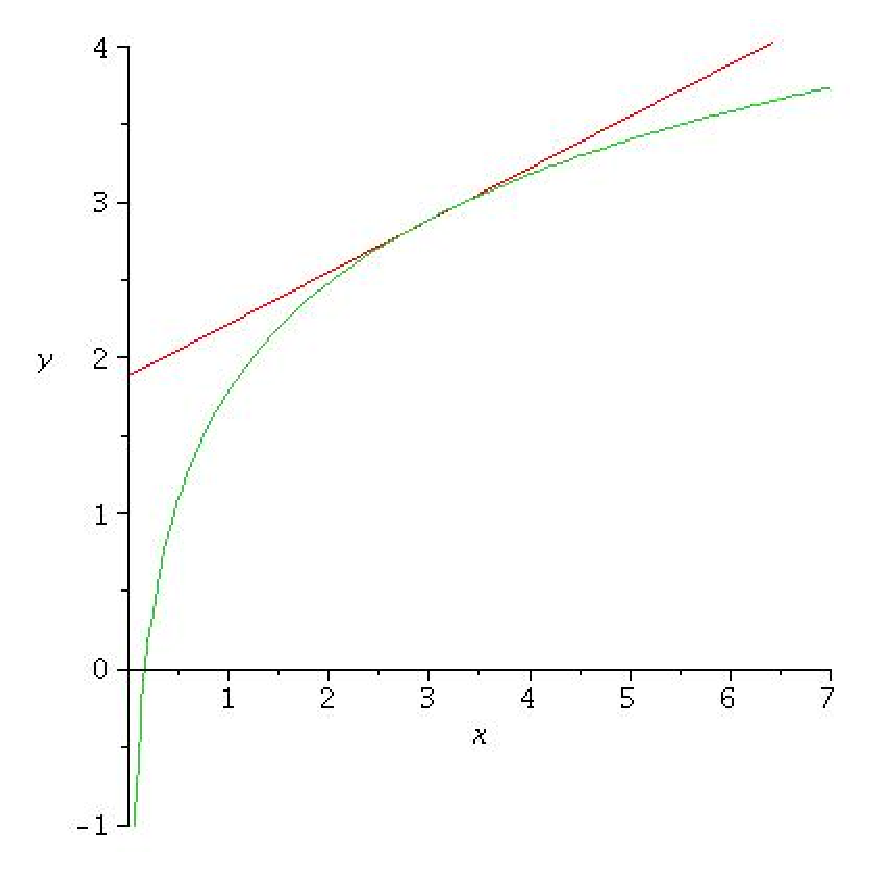
\includegraphics[width=0.5\textwidth]{grafica2.eps}
     \caption{Centrado en 6, de grado 2}
     \label{fig:ejemplo}   
  \end{center}
\end{figure}
\end{frame}

%%%%%%%%%%%%%%%%%%%%%%%%%%%%%%%%%%%%%%%%%%%%%%%%%%%%%%%%%%%%%%%%%%%%%%%%%%%%%%%%%%%%%%%%%%

\subsection{Resultados obtenidos 4}
\begin{frame}
\frametitle{Gráfica 2}
\begin{figure}
 \begin{center}
     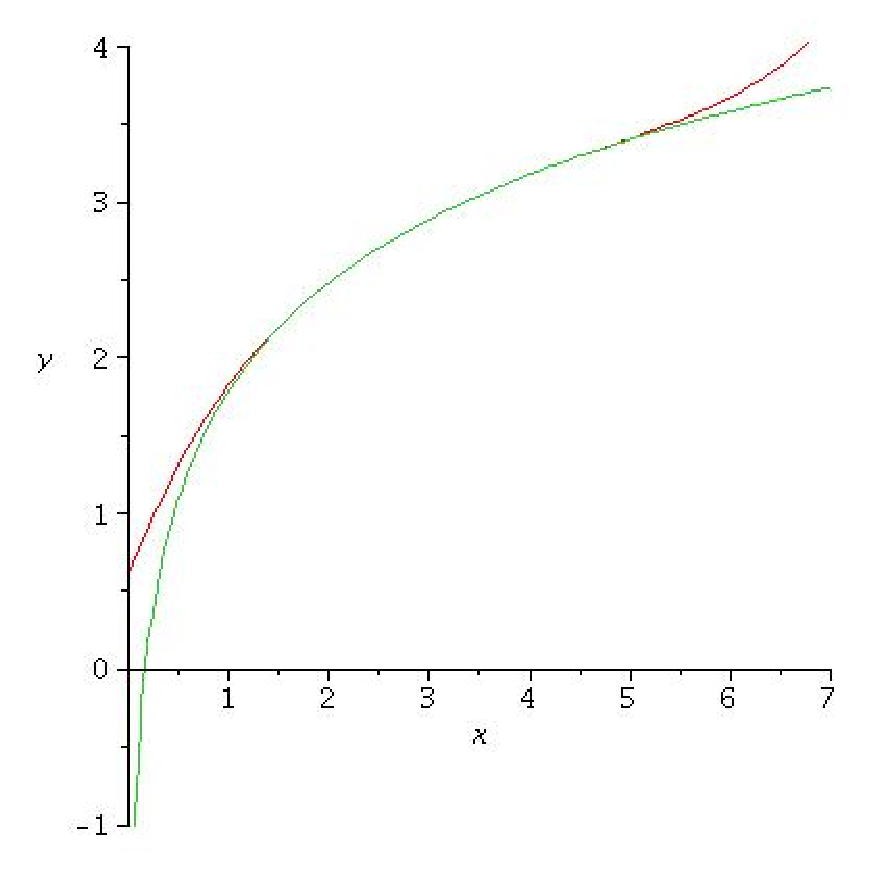
\includegraphics[width=0.5\textwidth]{grafica6.eps}
     \caption{Centrado en 6, de grado 6}
     \label{fig:ejemplo2}     
 \end{center}
\end{figure}
\end{frame}


%%%%%%%%%%%%%%%%%%%%%%%%%%%%%%%%%%%%%%%%%%%%%%%%%%%%%%%%%%%%%%%%%%%%%%%%%%%%%%%%%%%%%%%
\section{Conclusiones}
\subsection{Conclusiones}
\begin{frame}
\frametitle{Conclusiones}

\begin{itemize}

 \item Las series de Taylor, dependiendo de la naturaleza de la función, pueden llevar asociados un error, que tenderá a cero si tomamos una
 función lo suficientemente buena como pueden ser: $\sen(x)$, $\cos(x)$, $ln(x)$, \ldots
 \item La aproximación de Taylor se aproxima tanto como queramos, poniendo una mayor cantidad de términos en el polinomio.
 \item Es una herramienta matemática que facilita mucho los cálculos de aproximación de funciones.
 \item Se puede programar rápidamente, ya que no es de gran complejidad. Sólo necesitamos un punto, un lugar donde centrar el polinomio y 
el grado que queremos. Ofrece resultados de manera muy precisa.
\end{itemize}
\end{frame}

%%%%%%%%%%%%%%%%%%%%%%%%%%%%%%%%%%%%%%%%%%%%%%%%%%%%%%%%%%%%%%%%%%%%%%%%%%%%%%%%%%%%%%%%%%%
\section{Algoritmos}
\subsection{Interpolador de Taylor}
\scriptsize
\begin{frame}[fragile]
\begin{verbatim}
#!/usr/bin/python
#Autores: Lorena Díaz Morales, Jennifer Cabrera Mesa, Claudio García Vargas
import sys
from math import *
def taylor(x,n,d):                                                                                                        
  subtotal=0                                                                                                              
  tot=0                                                                                                                   
  i=1                                                                                                                     
  while i<=n :                                                                                                            
   ti = ((((-1)**(i+1))*factorial(i-1))/((x**i)*(factorial(i))))*((x-d)**i)                                               
   subtotal = float(subtotal)+float(ti)                                                                                   
   i+=1                                                                                                                   
  valor = float(log(6*d))
  tot = float(valor) + float(subtotal)
  return tot
if __name__=='__main__':
  x = float(sys.argv[1])
  n = int(sys.argv[2])
  d = float(sys.argv[3])
  print 'La aproximacion de Taylor es',taylor(x,n,d)
  diferencia=float(float(log(6*x))-float((taylor(x,n,d))))
  l=float(log(6*x))
  print 'La diferencia entre el valor real  interpolacion es',diferencia
  print 'Valor de la funcion orignial en el punto:',l
\end{verbatim}
\end{frame}

%%%%%%%%%%%%%%%%%%%%%%%%%%%%%%%%%%%%%%%%%%%%%%%%%%%%%%%%%%%%%%%%%%%%%%%%%%%%%%%

\begin{frame}
\begin{center}
 \huge
    Fin de la presentación
\end{center}
\end{frame}

%%%%%%%%%%%%%%%%%%%%%%%%%%%%%%%%%%%%%%%%%%%%%%%%%%%%%%%%%%%%%%%%%%%%%%%%%%%%%%%

\end{document} 
